% One-page summary for the meeting with Oliver (and Meisam), 19 Oct 2026.
% Build: pdflatex meeting_1019_summary.tex (twice).
\documentclass[11pt,a4paper]{article}
\usepackage[margin=2cm]{geometry}
\usepackage{amsmath,amssymb}
\usepackage{mathptmx}
\usepackage{enumitem}
\usepackage{graphicx}
\usepackage{tabularx,booktabs}
\graphicspath{{assets/}}
\setlist{nosep,leftmargin=*}
\pagestyle{empty}
\begin{document}
\begin{center}
{\large\bfseries Coupling the field and the point model at the Gauss points}\\[2pt]
Keisuke Nishioka, meeting on 19 October 2026
\end{center}

\paragraph{Where I am.} The thesis is written; I plan to submit in mid-November
(colloquium 16 December). The point model is
the Hamilton point model of Klempt et al., with the interaction parameters
calibrated by Bayesian inference (TMCMC) on the in-vitro data of Heine et al.;
it is not machine-learning based.

\paragraph{1. $\phi_{3D}$ at the quadrature points.} The element solves the field
by the NEM directly at the Gauss points and the surface points, so $\phi_{3D}$ is
available at each Gauss point without interpolation. The point model is solved
at every Gauss point next to the field.

\paragraph{2. The two voids: two schemes implemented.}
\begin{itemize}
\item \emph{Scaled.} The field sets the amount, the point model only the
  composition $\phi_i/\sum_j\phi_j$ and $\psi_i$. At each Gauss point and substep
  the point-model state is scaled to $\sum_i\phi_i=\phi_{3D}$, advanced and scaled
  again. This sets $\phi_0=1-\phi_{3D}$, i.e.\ it gives $\phi_0$ a physical meaning.
  When the field's amount equals the point model's own, the composition of the
  point model alone is recovered (to $10^{-5}$ or better).
\item \emph{Unscaled.} $\phi_0$ stays auxiliary: the point model runs on its own from
  the moment the field reaches a threshold and supplies only the composition.
\end{itemize}
The composition then depends on the local amount (scaled) or on the local age of
the biofilm (unscaled).

\noindent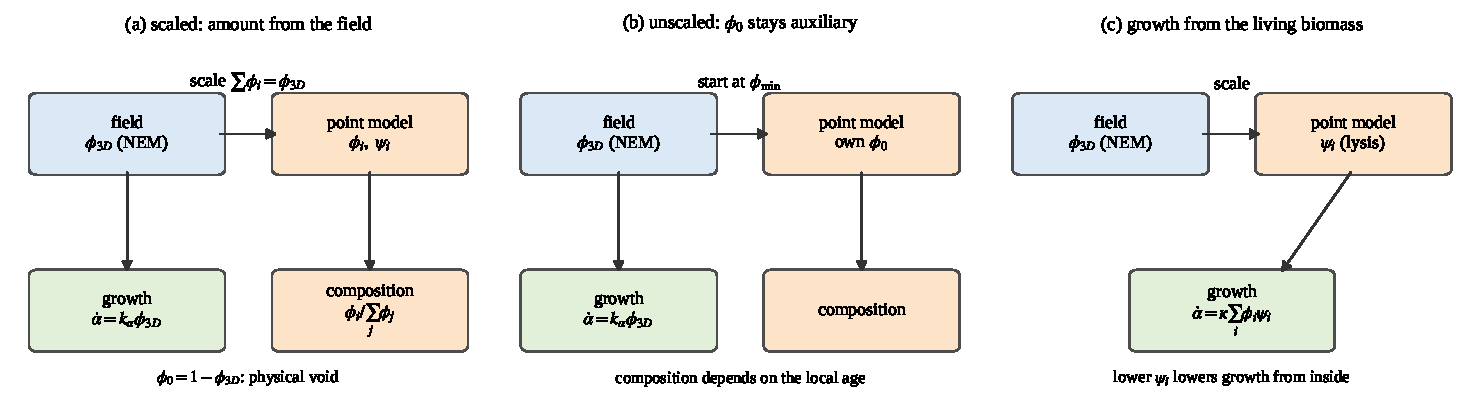
\includegraphics[width=\linewidth]{fig_meeting1019_schemes.pdf}\\
{\small Coupling at a Gauss point: (a) scaled and (b) unscaled scheme, (c) growth from the living biomass of the point model.}

\paragraph{3. Lysis acting on growth.} In a first run with the calibrated
five-species model, $\alpha$ grows with the living biomass $\sum_i\phi_i\psi_i$ of
the point model instead of with $\phi_{3D}$. A drop of $\psi_i$ (lysis, or an
antibiotic in the point model) then lowers the growth from inside the point
model. With the rate chosen so that the mean growth equals that of Eq.~36, the
mean von Mises stress of the seed changes by $8\,\%$. With an antibiotic in the
point model (same sensitivity for all five species, strength chosen so that the
living fraction halves by $T^*=1$; both assumed), scheme (c) gives $26\,\%$ less
growth and $32\,\%$ less seed stress, while scheme (a) gives the same stress as
without the antibiotic, only the composition changes. The growth and the stress
are proportional to $\kappa$. The rates are my choice, not from a paper.

\noindent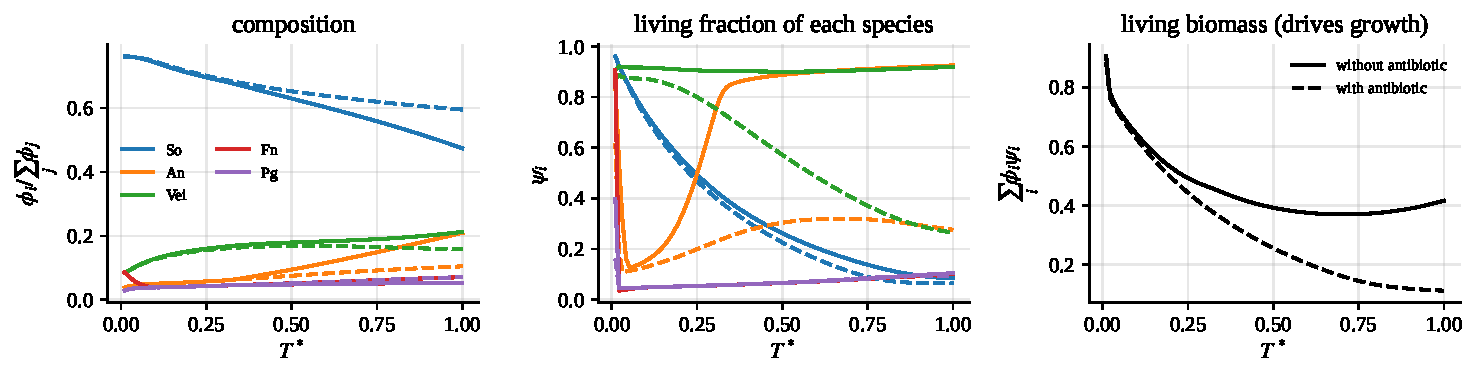
\includegraphics[width=\linewidth]{fig_meeting1019_lysis_trace.pdf}\\
{\small Point model at a seed Gauss point, scheme (c), without (solid) and with (dashed) the antibiotic, applied at a constant level from $T^*=0$.}

\noindent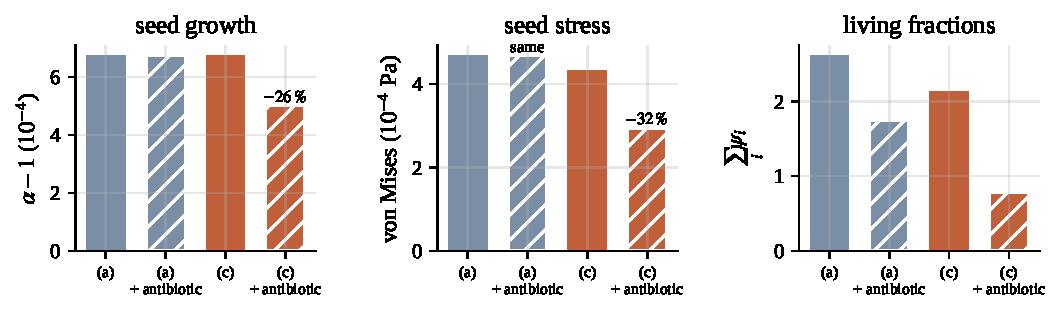
\includegraphics[width=\linewidth]{fig_meeting1019_lysis.pdf}\\
{\small Antibiotic in the point model (commensal flow condition, $8^3$, $T^*=1$, means over the seed elements): (a) growth from $\phi$ of the field, (c) growth from the living biomass.}

\noindent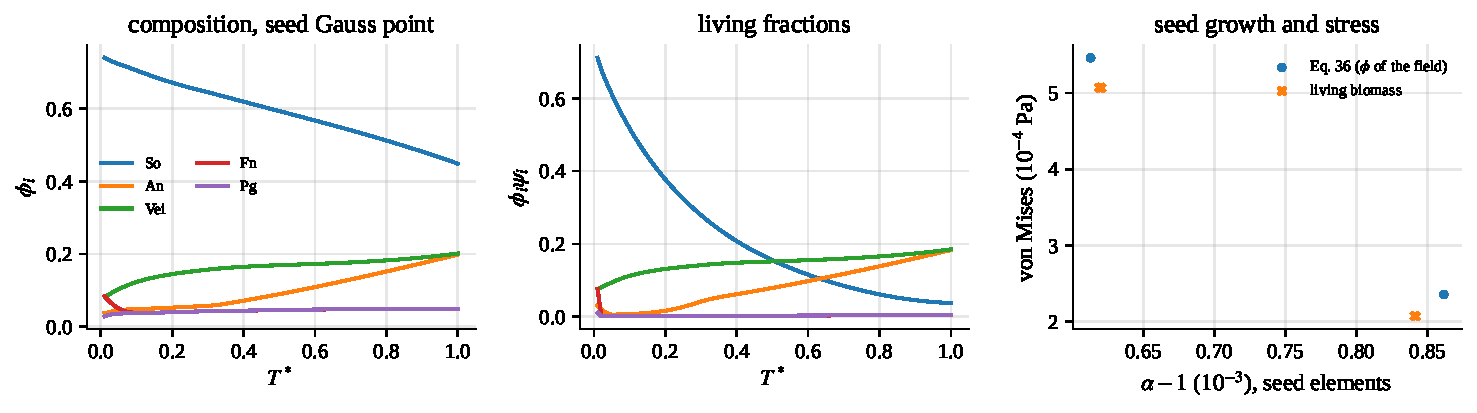
\includegraphics[width=\linewidth]{fig_meeting1019_cal5.pdf}\\
{\small Calibrated five-species model in the element (commensal flow condition, $8^3$, $T^*=1$): composition and living fractions at a seed Gauss point; growth and stress of the seed elements for Eq.~36 and for growth from the living biomass.}

\par\noindent\begin{minipage}{\linewidth}
\paragraph{Comparison and proposal.}
\begin{center}\small
\begin{tabularx}{\linewidth}{@{}l>{\raggedright\arraybackslash}X>{\raggedright\arraybackslash}X>{\raggedright\arraybackslash}X@{}}
\toprule
& (a) scaled & (b) unscaled & (c) growth from living biomass\\
\midrule
What it does & amount from the field, composition from the point model, scaled to $\sum_i\phi_i=\phi_{3D}$ & point model runs on its own, supplies the composition only & as (a), but $\dot\alpha=\kappa\sum_i\phi_i\psi_i$\\
Meaning of $\phi_0$ & physical void, $1-\phi_{3D}$ & auxiliary, as in the paper & as (a)\\
Composition depends on & local amount & local age of the biofilm & local amount\\
Lysis acts on growth & no & no & yes, lower $\psi_i$ lowers growth\\
Check & recovers the point model alone to $10^{-5}$ & point-model trajectory, shifted in time & $8^3$: seed stress $-8\,\%$; with antibiotic $-32\,\%$, (a) unchanged\\
In the thesis & Chapter 4 & Chapter 4, for comparison & Outlook, one paragraph\\
Strength & well tested, simple to explain & closest to the paper's reading of $\phi_0$ & answers the lysis question; growth from the producing biomass has precedent in the literature\\
Weakness & gives $\phi_0$ a physical meaning (stated as an assumption) & nearly decoupled from the field; cannot feed lysis back & $\kappa$ is my choice; $8^3$ only so far\\
\bottomrule
\end{tabularx}
\end{center}
\noindent\emph{Proposal:} (a) as the basis, (c) as its extension to let lysis act on
growth, and (b) kept as a comparison for the interpretation of $\phi_0$.
\end{minipage}

\paragraph{4. Limits stated in the thesis.} The coupling is one-way for the
mechanics (the composition does not change the stiffness). The scaled scheme
gives $\phi_0$ a meaning the point model does not intend. A coupling without
these choices would need a spatial multispecies model from one variational
principle. A recent check: the value of $\phi$ at the surface points is a mean of
neighbouring Gauss points, exact only for constant fields, so the Laplacian next
to a face has an error that does not decrease with the mesh; in my seed runs this
layer carries $0.1$ to $0.2\,\%$ of the error.

\paragraph{Ideas for experiments (to plan together).}
\begin{enumerate}
\item \emph{Two antibiotics during growth.} Add an antibiotic at a constant
  concentration to the five-species biofilm of Heine et al.\ partway through
  (as in the validation case of Fritsch et al.), once a broad one
  (chlorhexidine) and once one that acts on the anaerobes (metronidazole:
  \textit{V.~dispar}, \textit{F.~nucleatum}, \textit{P.~gingivalis}, less on
  \textit{S.~oralis} and \textit{A.~naeslundii}); measure the live fraction
  (LIVE/DEAD) and the biofilm volume (CLSM). Scheme (c) predicts that the volume
  growth slows when the dominant species is hit, so differently for the two drugs
  and for the commensal and the dysbiotic community; scheme (a) predicts no
  change of the volume for either. This decides between them.
\item \emph{Co-culture without Fn.} Grow the dysbiotic community under flow without
  \textit{F.~nucleatum}. The calibrated model predicts that the late increase of
  \textit{P.~gingivalis} disappears.
\item \emph{Spatial composition.} Depth profiles of the species by FISH and CLSM
  (partly available at NIFE). Composition set by the local amount (a) or by the
  local age (b) gives different profiles; this bears on the meaning of $\phi_0$.
\item \emph{Stiffness.} Young's modulus by AFM per condition or per community
  (as in Pattem et al.\ 2018), replacing the assumed $E=10$~Pa; a dependence on
  the composition would support a two-way coupling.
\item \emph{Growth-induced deformation.} Biofilm grown on a soft substrate (gel or
  thin membrane); the measured deformation gives the growth-induced stress, the
  closest available check of the stresses.
\end{enumerate}
Items 1 and 2 extend the existing culture system and could be done first; 1 and 4
would also serve your deterministic model.

\paragraph{To decide together.}
\begin{enumerate}
\item \emph{Meaning of $\phi_0$.} I would keep scheme (a) as the basis and state
  $\phi_0=1-\phi_{3D}$, the void of the field, as an assumption, with scheme (b)
  as a comparison. It is the simpler reading to explain and the one under which
  lysis can act on growth through scheme (c). Do you agree, or would you rather
  keep $\phi_0$ auxiliary as in the paper?
\item \emph{Experiments.} I would start with items 1 and 2, because they extend
  the existing culture system of Heine et al.\ and test the two predictions
  directly. Would these also be useful for your work, and should I contact
  N.~Heine and colleagues at MHH or someone else first?
\end{enumerate}
\end{document}
